\chapter{Known Vulnerabilities \& Misconfigurations in Docker}
In this chapter we will look at Docker from a vulnerability analysis perspective. First we will look conceptually at Docker and security by examining the attack surface of Docker on an host and the various attacker models that come with it.
We then look at some interesting, practical examples of security problems of Docker. These are split into vulnerabilities and misconfigurations.

\hfill

Vulnerabilities and misconfigurations are both security problems, but they differ in who made the mistake. A vulnerability is a problem in a program itself. For example, a buffer overflow is a clear vulnerability. The problem lies solely in the program itself. To fix it, the code of the program needs to be changed.

Misconfigurations, on the other hand, are security problems that come from wrong usage of a program. The program is incorrectly configured and that creates a situation that might be exploitable to an attacker. For example, a world-readable file containing passwords is a misconfiguration. To fix a misconfiguration, the user should change the configuration of the problem. The developers of the program can only recommend users to configure it correctly (and have documentation on how to do it).

\section{Attack Surface \& Models}
\todo[inline]{Does docker increase/decrease the attack surface of an host}
\todo[inline]{Does docker increase/decrease the impact/likelihood of an exploit?}
\todo[inline]{\url{https://docs.docker.com/engine/security/security/}}

Because Docker is more of an ecosystem than a single running process, it has quite a large attack surface. This attack surface consists of multiple attacker models.

\hfill

Lets take a look at the following image.

\begin{figure}[ht]
    \centering
    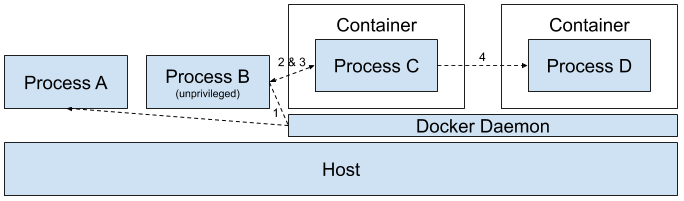
\includegraphics[width=.8\linewidth]{resources/images/attacksurfaces.png}
    \label{} 
\end{figure}

We see four distinct processes:
\begin{enumerate}
    \item[A)] A standard (privileged) process running directly on the host. 
    \item[B)] A standard unprivileged process running directly on the host.
    \item[C)] A process running in a Docker container.
    \item[D)] Similar to C. 
\end{enumerate}

\hfill

We also see four distinct attacker scenarios/models:
\begin{enumerate}
    \item[1)] An unprivileged process accessing privileged data (in the image process A) using the Docker Daemon.
    \item[2)] An unprivileged process accessing data in a Docker container.
    \item[3)] A Docker container accessing data on the host (that it should not be able to access).
    \item[4)] One container accessing data in another container. 
\end{enumerate}

\subsection{Container Escapes}
One of the most prominent types of vulnerability (and sometimes misconfiguration) is the possibility for a process running in a container to escape the container and access data on the host.

\hfill

An example attack scenario would be a company that offers a PaaS (Platform as a Service) products that allows customers to run dockers on their infrastructure\footnote{This is actually quite common nowadays. All major computing providers offer such a service.}. If it is possible for the attacker to submit a Docker image that escapes the container and access the underlying infrastructure, they could access other containers or even other internal resources. That would, obviously, be a very big problem for that company.

\hfill

As noted before, because a container usages the same kernel and resources as the host; an exploit granting root can be just as devastating run inside as outside of the docker, because the target kernel and resources are the same.

It should also be noted that an exploit that allows someone to escape from a Linux \lstinline{namespace} is essentially a container escape exploit. CVE--2017--7308\cite{cve20177308} is a good example of this.

\subsection{Docker Daemon}
\todo[inline]{attacks host $\to$ container $\to$ host}
\todo[inline]{host (unprivileged) $\to$ docker}
\todo[inline]{\href{https://github.com/docker/engine/blob/v19.03.0-rc3/docs/rootless.md}{Rootless mode (Experimental)}}

\subsection{Container to Container}
\todo[inline]{attacks container $\to$ container}

\subsection{Deployment \& Development Pipelines}
One of the biggest usages of Docker is automating part of the deployment and development process. 

\subsection{The impact of Docker on existing vulnerabilities}
A Docker container isolates software from the host, but does not change it. This means that vulnerabilities in software are not affected by Dockerizing that software. However, the impact of those vulnerabilities is decreased, because the vulnerability exists in a isolated environment.

If, for example, there exists a RCE (remote code execution) vulnerability in Wordpress. Running Wordpress in a Docker container does not fix the vulnerability. An attacker is still able to exploit it. But that attacker is not able to access the host system, because the exploited software is isolated from the host system because of Docker. 

\subsection{Protection Mechanisms}
\todo[inline]{SELinux}
\todo[inline]{AppArmor}
\todo[inline]{Secure Computing Mode Profiles}
\todo[inline]{\url{https://github.com/genuinetools/bane}}

\section{Vulnerabilities}
\todo[inline]{CVSS}
\todo[inline]{Link to attack scenario}

In the \hyperref[appendix:CVE-List]{appendix} you can find a list of all the Docker related vulnerabilities I have looked at.

\subsection{\texorpdfstring{\lstinline{waitid()}}{waitid()} Container Escape (CVE--2017--5123)}
\todo[inline]{CVE--2017--14954}
\todo[inline]{Kernel exploit}

\subsection{Alpine Image Root Password (CVE--2019--5021)}
\begin{lstlisting}
$ docker run -it --rm alpine:3.5 cat /etc/shadow
root:::0:::::
\end{lstlisting}

\begin{lstlisting}
(host)$ docker run -it --rm alpine:3.5 sh
(cont)# apk add --no-cache linux-pam shadow
...
(cont)# adduser test
...
(cont)# su test
Password:
(cont)$ su root
(cont)#
\end{lstlisting}

This vulnerability has a CVSS score of 9.8 (and a 10 in CVSS 2)\footnote{\url{https://nvd.nist.gov/vuln/detail/CVE-2019-5021}}. The CVSS scores are out of 10, meaning this is seen as an extremely high-risk vulnerability. But in actuality, this vulnerability is only risky in very specific cases. "Empty \lstinline{root} password" sounds very dangerous, but it really is not that dangerous in an isolated container that runs root by default. Only in the very specific case that a process in a container runs as a non-root user and their is some vulnerability or misconfiguration that allows \lstinline{root} to escape the container and an attacker can get control of the process in the container is this dangerous. In other words, this vulnerability is actually not likely to be used in the wild and most likely needs to be combined with another vulnerability or misconfiguration to be able to do damage.

\subsection{\texorpdfstring{\lstinline{runC}}{runC} Container Escape (CVE--2019--5736)}

\section{Misconfigurations}
\todo[inline]{\href{https://neoteric.eu/blog/docker-containers-with-root-privileges/}{Docker containers with root privileges}}
\todo[inline]{\url{https://www.katacoda.com/courses/docker-security/}}
\todo[inline]{Permissions on config/service files}
\todo[inline]{Wrong volumes: / or /proc}
\todo[inline]{Non-docker group Docker access?}
\todo[inline]{Research: create user and group in Dockerfile}
\todo[inline]{Map to CIS Benchmark}
\todo[inline]{Does CIS cover everything?}
\todo[inline]{\href{https://www.nccgroup.trust/uk/our-research/abusing-privileged-and-unprivileged-linux-containers/}{Abusing Privileged and Unprivileged Linux Containers}}
\todo[inline]{\href{https://www.nccgroup.trust/uk/our-research/understanding-and-hardening-linux-containers/}{Understanding and Hardening Linux Containers}}
\todo[inline]{\href{https://0x00sec.org/t/securing-docker-containers/16913}{Securing Docker Containers}}
\todo[inline]{\href{https://www.reddit.com/r/docker/comments/dkgtfv/10_docker_image_security_best_practices/}{10 Docker Image Security Best Practices}}
\todo[inline]{\href{https://www.exploit-db.com/exploits/42650}{Docker Daemon - Unprotected TCP Socket (Metasploit)}}
\todo[inline]{\href{https://www.redhat.com/en/blog/secure-your-containers-one-weird-trick}{Linux Capabilities: Secure Your Containers with this One Weird Trick}}
\todo[inline]{\url{http://training.play-with-docker.com/security-seccomp/}}

\subsection{The -{}-privileged flag}
\todo[inline]{\href{https://blog.trailofbits.com/2019/07/19/understanding-docker-container-escapes/}{Understanding Docker container escapes}}

\subsection{Root user}
\todo[inline]{\href{http://www.projectatomic.io/blog/2016/01/how-to-run-a-more-secure-non-root-user-container/}{How to Run a More Secure Non-Root User Container}}

